\documentclass[12pt,a4paper]{article}
\usepackage[top=25.4mm, bottom=25.4mm, left=19.1mm, right=19.1mm]{geometry}


\usepackage[latin2]{inputenc}
\usepackage{graphicx}
\graphicspath{ {./images/} }
\usepackage{ulem}
\usepackage{amsmath}
\usepackage[document]{ragged2e}

\setlength{\parindent}{4em}
\setlength{\parskip}{1em}
\usepackage{hyperref}

\usepackage{fancyhdr}
\pagestyle{fancy}
\fancyhf{}
\fancyhead[LO]{\textbf{\small IoT and Smart Analytics}\\
\text{\small A Program by IIITH and TalentSprint}}

\usepackage{xcolor}
\usepackage{lipsum}

\rhead{\begin{picture}(0,0) \put(-250,-2){
\includegraphics[width=9cm]{EXP_06_Images/ts-iisc-logo-pr.png}} \end{picture}}
\cfoot{\thepage}


\begin{document}

\begin{center}

\textbf{\large \\EXPERIMENT 06 }\\[6pt]
\text{ Introduction to ESP32   }
\end{center}

\textbf{\large LEARNING OBJECTIVES:}\\[3pt]
At the end of this experiment, participants will be able to:\vspace{-6mm}\begin{enumerate}
 \setlength\itemsep{-0.3em}
\item Understand input/output pins and their functions in ESP32 \\
\item Implement LED blinking with ESP 32 board 
\end{enumerate}
\textbf{\large APPARATUS REQUIRED:}\\
\vspace{-3mm}
\begin{enumerate}
 \setlength\itemsep{-0.3em}
\item ESP32 Module-1pcs \\
\item USB cable-1pcs\\
\item Arduino IDE
\end{enumerate}

\begin{justify}
\textbf{\large THEORY}\\[3pt]
\textbf{Introduction}: ESP32 is a low-cost System on Chip (SoC) Microcontroller from Espressif Systems, the developers of the famous ESP8266 SoC. ESP32-WROOM-32 is a generic module integrating Wi-Fi+BT+BLE MCU and targets various applications from low-power sensor networks to the most demanding tasks. It comes in both dual-core and single-core versions, which has WiFi and Bluetooth inbuilt. It runs 32-bit programs, and the clock frequency can go up to 240 MHz and has 512 Kb RAM. It has a variety of peripherals like capacitive touch, ADCs, DACs, UART, SPI, I2C, and much more. Fig.1 below shows the pinout diagram of the 30 – pin version of the ESP32 Development Board (which is provided in our Kit). For more specifications, refer to the \href{https://www.electronicshub.org/getting-started-with-esp32/}{link.}\\
Let’s look at the different components of the ESP32 board as given in fig.2. It has a few buttons and LEDs where the Power LED (Red) indicates the power supply that will glow when the board is powered. The other LED (Blue) is connected to the GPIO pin that can be controlled through programming.\\
\textbf{The ESP32 can be programmed using many programming environments. A few of them are:}\
\begin{itemize}
  \item Lua
  \item Micropython
  \item Espressif IDF
  \item Javascript
  \item Arduino IDE
\end{itemize}
\setlength{\parindent}{0eM}
Each of the programming environments requires the corresponding setup. For our purpose, we will use Arduino IDE in the following experiments. We need to install an add-on for the IDE to use the Arduino IDE for programming the ESP32 module.\end{justify}


\begin{center} 
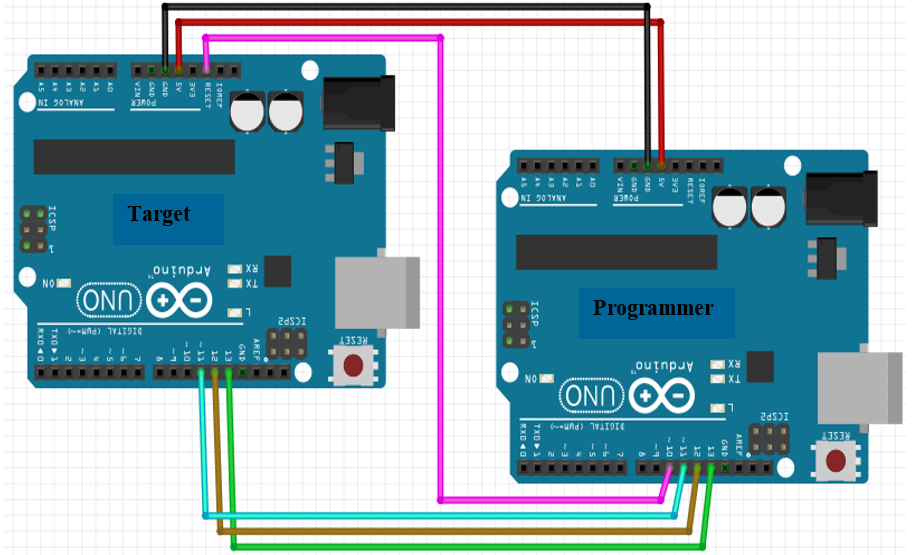
\includegraphics[scale=0.7]{EXP_06_Images/fig1.png}
\end{center}
\begin{center} {Figure 1. ESP32 WROOM32 board Pin labels [1]}\end{center}
\begin{center} 
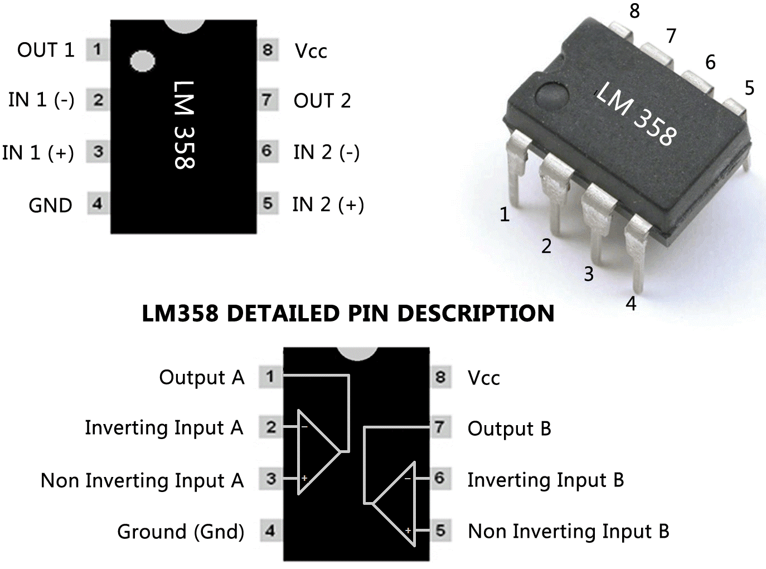
\includegraphics[scale=0.45]{EXP_06_Images/fig2.png}
\end{center}
\begin{center} {Figure 2. ESP32 -WROOM-32 [1]}\end{center}

\setlength{\parindent}{0eM}
\\[21pt]\textbf{\large PROCEDURE}\\[6pt]
\textbf{Installing and setting up ESP32 on Arduino IDE:}To install the ESP32 board add-on on Arduino IDE, follow the instructions given below:

\begin{enumerate}
\setlength\itemsep{-0.3em}
\item{In the IDE, go to FILE  \rightarrow  PREFERENCES}\\

\item{Add \textbf{https://dl.espressif.com/dl/package\_esp32\_index.json} in the Additional Board Manager URLs field and click the ok button.}

\begin{center} 
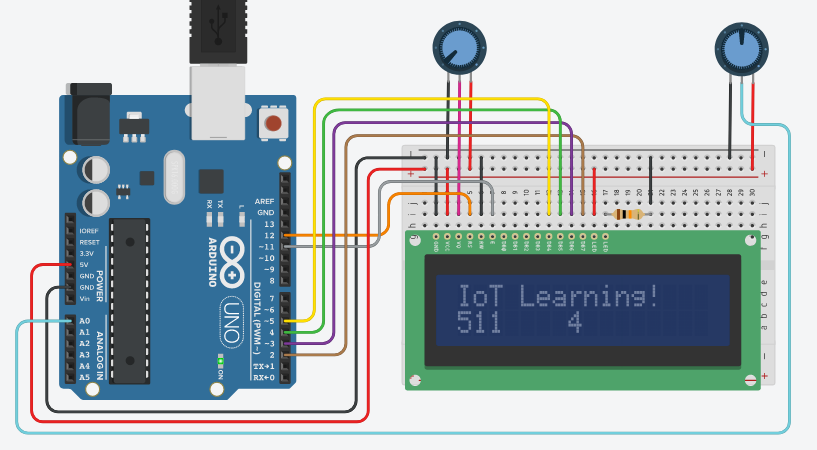
\includegraphics[scale=0.85]{EXP_06_Images/fig3.png}
\end{center}
\begin{center} {Figure 3. Additional boards}\end{center}
\textbf{Note:} If there are already boards URL, you can separate the URLs with a comma as shown.

\item{ Open the boards manager by going to TOOLS$\rightarrow$  BOARD $\rightarrow$BOARDS MANAGER.}

\item{In the boards manager, search for ESP32 and install ESP32 by Espressif Systems.}

\begin{center} 
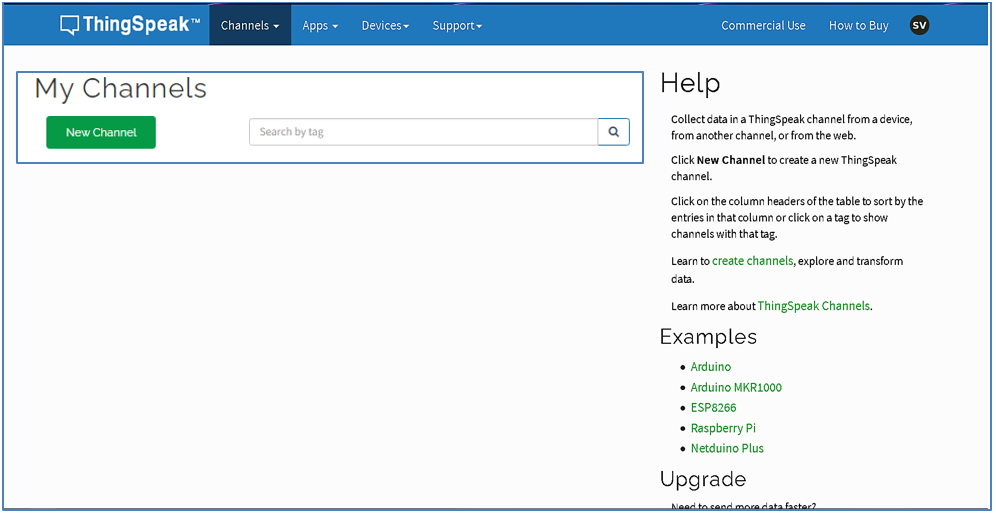
\includegraphics[scale=0.85]{EXP_06_Images/fig4.png}
\end{center}
\begin{center} {Figure 4. Board Installation }\end{center}


\item Following the above steps should install the board. Now we can select the ESP32 board as shown in Fig 4.
\begin{center} 
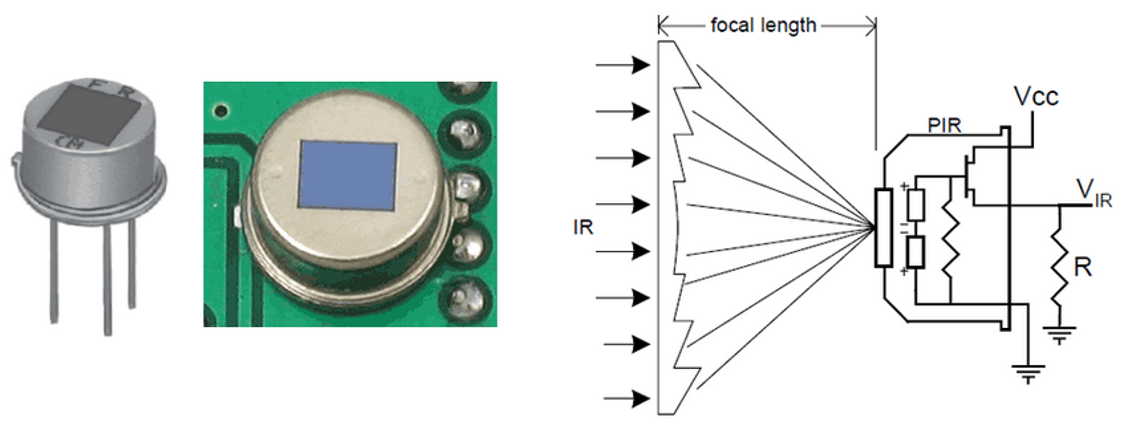
\includegraphics[scale=0.85]{EXP_06_Images/fig5.png}
\end{center}
\begin{center} {Figure 5. Board selection}\end{center}

\item Select the corresponding port. By the end of this step, your ESP32 is ready to be programmed.

\end{enumerate}


\setlength{\parindent}{0eM}
\textbf{Hardware/software setup :} In this experiment, we will blink the inbuilt LED of the ESP32 board using Arduino IDE. We can also control some external LEDs by connecting them with the ESP32 board to understand the working of the GPIO pins. Similar to Arduino Uno board programming, we can program the ESP32 board.
Follow the steps given below for LED blinking:
\begin{enumerate}
 \setlength\itemsep{-0.3em}
 
\item {Connect the ESP32 board to the computer using a micro-USB cable. The RED LED will glow, which indicates that the board is powered.}

\item{Go to Tools $\rightarrow$ Board from the top menu and click on the 'ESP32 Arduino' option. Then select the ESP32 board type, i.e., ESP32 dev module.}

\item{Now go to Tools $\rightarrow$ Port, and select the port to which the board is connected.}

\item{Write the ESP32 board blinking LED program given below.}

\item{Click the upload option to upload your LED blinking code. If not connecting, then press and hold the BOOT button during the uploading process.}
\end{enumerate}


\hspace{2cm}\textbf{\large Code:}\\[6pt]

\setlength{\parindent}{10eM}\\

\textcolor{blue}{// Define the inbuilt LED pin}\\
\#define LED\_PIN 2 \\[3pt]
void setup() \\
\textcolor{blue}{//Initialize GPIO pin 2 LED PIN as an output}\\[3pt]
\{\\
pinMode(LED\_PIN, OUTPUT);\\
\}\\[3pt]
void loop()\\
\{\\
\textcolor{blue}{//turn the LED on}\\
digitalWrite(LED\_PIN, HIGH);\\
\textcolor{blue}{// wait for a second}\\
delay(1000);\\
\textcolor{blue}{//turn the LED off}\\
digitalWrite(LED\_PIN, LOW);\\
\textcolor{blue}{//wait for a second}\\
delay(1000);\\
\}\par

\setlength{\parindent}{0eM}
\begin{justify}\textbf{Explanation of Arduino Program:} Define Pin 2 with a macro called LED\_PIN. Whenever the name LED\_PIN appears in the program, the compiler changes it to pin no. 2. So, to use a pin other than GPIO pin 2, you have to replace the GPIO PIN where you defined the macro for GPIO pin 2.
An Arduino program generally has two sections: \textbf{void setup()} and \textbf{void loop()}:\\[3pt]
\underline{void setup():}\\[6pt]
pinMode(LED\_PIN, OUTPUT);\\[3pt]
Here, we are initializing the mode of the LED\_PIN GPIO pin as OUTPUT.\\[3pt]
\underline{void loop():}\\[6pt]
digitalWrite(LED\_PIN, HIGH);\\[3pt]
delay(1000);\\[6pt]

\noindent In the loop() function, we use the digitalWrite() function to set the GPIO pin to HIGH. It will set the GPIO pin 2 to 5 Volts, and the inbuilt LED will turn ON. Then we used a delay() function that will stop the program execution for 1000 milliseconds (1 second).

\noindent digitalWrite(LED\_PIN, LOW);\\[3pt]
delay(1000);\\[6pt]

\noindent The digitalWrite() function is used again to set the GPIO pin to LOW. It will set the GPIO pin 2 to 0 Volts, and the inbuilt LED connected will turns OFF. Another delay() function stops the program execution for 1000 milliseconds (1 second).\end{justify}

\begin{center} 
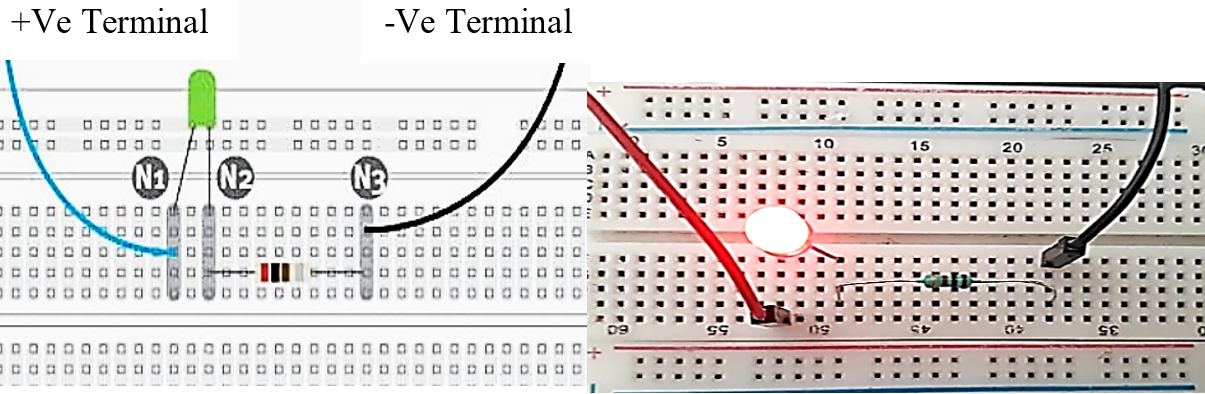
\includegraphics[scale=0.8]{EXP_06_Images/fig6.png}
\end{center}
\begin{center} {Figure 6. Inbuild  LED blinking}\end{center}


\setlength{\parindent}{0eM}
\textbf{\large REFERENCES:}
\vspace{-6mm}
\begin{enumerate}
\setlength\itemsep{-0.3em}
 \item  \href{https://www.electronicshub.org/getting-started-with-esp32/}{Getting Started with ESP32}
\item   \href{https://www.espressif.com/sites/default/files/documentation/esp32-wroom-32_datasheet_en.pdf}{ESP32-WROOM Datasheet}
\end{enumerate}

\textbf{\large CONCEPT DRILLS:}
\vspace{-6mm}
\begin{enumerate}
 \setlength\itemsep{-0.3em}
\item Design a circuit using  ESP32, LED, and Push Button and write the appropriate program so that LED glows only while the push-button is triggered. Use the concept of digital read.
\item Design a dimmable LED using  ESP32 and Potentiometer with the appropriate program. 
\item Simulate Logic gates using ESP32. The program should be user interactive i.e. appropriate messages should be displayed on the serial monitor.
\end{enumerate}
\end{document}